% content goes here 

\section{Intro}
\begin{frame}
	\frametitle{Intro}

	\begin{columns}[c]
    	\column{.5\textwidth} 
        	\begin{itemize}
            	\item Operating Systems:
                \begin{itemize}
            		\item Windows
                    \item macOS
                    \item Linux
            	\end{itemize}
                \item Computer Science UA: Linux
            \end{itemize}
            \begin{itemize}
                \item Use Linux:
                \begin{itemize}
            		\item Virtual Machine
                    \item Boot
                    \item Dual Boot
            	\end{itemize}
            \end{itemize}
        \column{.5\textwidth}
            \centering
			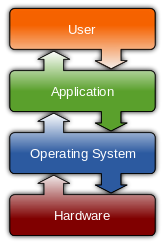
\includegraphics[width=.7\linewidth,]{res/os}
    \end{columns}

	\note{
    	\begin{itemize}
        	\item OS bouwt op hardware. Applicaties bouwen op OS.
            \item Taken, projecten, examens $\rightarrow$ Linux
            \item Boot simpel geval van dual boot
        \end{itemize}
    }
	
\end{frame}

\section{Distros}
\begin{frame}
	\frametitle{Linux Distributions - Distros}
	%\framesubtitle{}

	\begin{itemize}
		\item Linux = Free Open Source OS
        \item \href{https://upload.wikimedia.org/wikipedia/commons/1/1b/Linux_Distribution_Timeline.svg}{A lot of Forks} $\rightarrow$ Linux Distribution
	\end{itemize}
    \begin{itemize}
        \item \hyperlink{ubuntu}{Ubuntu}
        \item \hyperlink{ubuntu_gnome}{Ubuntu Gnome}
	\end{itemize}
\end{frame}

\begin{frame}[label=ubuntu]
	\frametitle{Ubuntu $ $ Ubuntu Gnome}
    Ubuntu
	\begin{itemize}
		\item Standard distribution (Unity)
		\item Installed on lab pc's
	\end{itemize}
    \vspace{0.5cm}
    Ubuntu Gnome
    \begin{itemize}
		\item Ubuntu Flavour
		\item Different Desktop Environment
	\end{itemize}
\end{frame}

\section{Virtual Machine}
\begin{frame}
	\frametitle{Virtual Machine}

    \begin{itemize}
    	\item Software to emulate a real machine
        \item Run OS within guest OS.
    \end{itemize} \vspace{0.5cm}
    
    Pros and Cons \vspace{0.1cm}
    \hrule 
    \begin{columns}[c]
    	\column{.5\textwidth}
            \begin{enumerate}
            	\item[$+$] Easy
                \item[$+$] Good  to try out OS
            \end{enumerate}
        \column{.5\textwidth}
            \begin{enumerate}
            	\item[$-$] Slow
                \item[$-$] Not reliable
            \end{enumerate}
    \end{columns} \vspace{0.5cm}

    \href{http://www.howtogeek.com/196060/beginner-geek-how-to-create-and-use-virtual-machines/}{Tutorial $\vcenter{\hbox{
\includegraphics[width=0.45cm]{res/link}}\vspace{0.1cm}}$} \\
        \href{https://www.virtualbox.org/}{Virtual Box $\vcenter{\hbox{
\includegraphics[width=0.45cm]{res/link}}\vspace{0.1cm}}$}
\end{frame}


\section{Dual Boot}
\begin{frame}
	\frametitle{Dual Boot}
    
    \begin{itemize}
    	\item Install OS alongside original OS.
    \end{itemize} \vspace{0.5cm}
    
    Pros and Cons \vspace{0.1cm}
    \hrule 
    \begin{columns}[c]
    	\column{.5\textwidth}
            \begin{enumerate}
           		\item[$+$] Fast
            	\item[$+$] Stable
                \item[$+$] Reliable
            \end{enumerate}
        \column{.5\textwidth}
            \begin{enumerate}
            	\item[$-$] Hard to set up
                \item[$-$] Can cause problems
                \item[$-$] Need reboot to switch
            \end{enumerate}
    \end{columns} \vspace{0.5cm}
    
    \href{http://www.ubuntu.com/download/desktop/install-ubuntu-desktop}{Tutorial $\vcenter{\hbox{
\includegraphics[width=0.45cm]{res/link}}\vspace{0.1cm}}$} \\
    \vspace{0.5cm}
    \textbf{Disclaimer:} We are not responsible for loss of data, broken laptops or hurt feelings. Dual boot is a dangerous activity, take precautions.
    
\end{frame}

\begin{frame}
	\frametitle{Dual Boot - Step 1}
 
 	Find distro:
    \begin{itemize}
    	\item \href{http://www.ubuntu.com/download}{Ubuntu $\vcenter{\hbox{
\includegraphics[width=0.45cm]{res/link}}\vspace{0.1cm}}$}
		\item \href{http://www.ubuntu.com/about/about-ubuntu/flavours} {Ubuntu Flavours $\vcenter{\hbox{
\includegraphics[width=0.45cm]{res/link}}\vspace{0.1cm}}$}
	\end{itemize}
    
\end{frame}

\begin{frame}
	\frametitle{Dual Boot - Step 2}
    
    Make bootable USB with ISO \\
    \href{http://www.ubuntu.com/download/desktop/create-a-usb-stick-on-windows}{Bootable USB Stick $\vcenter{\hbox{
\includegraphics[width=0.45cm]{res/link}}\vspace{0.1cm}}$} \\
    
\end{frame}

\begin{frame}
	\frametitle{Dual Boot - Step 3}
    
    Restart PC with USB plugged in.\\
    
    You might need to press F2/F12/DEL to change some BIOS options (If anything goes wrong):
 	\begin{itemize}
		\item Change boot order
		\item Disable secure boot
		\item Legacy boot?
	\end{itemize}
\end{frame}

\begin{frame}
	\frametitle{Dual Boot - Step 4}
    
    Follow installation instructions
    
\end{frame}

\begin{frame}
	\frametitle{Dual Boot - Step 5}
    
    If anything goes wrong, Google it or ask us.
    
\end{frame}

\begin{frame}
	\frametitle{Dual Boot - Step 6}
    
    Check if GRUB works by rebooting. If not, use boot-repair \\
    \href{https://help.ubuntu.com/community/Boot-Repair}{Boot-Repair $\vcenter{\hbox{
\includegraphics[width=0.45cm]{res/link}}\vspace{0.1cm}}$}
    
\end{frame}